\documentclass[tekniskrapport/tech.tex]{subfiles}

\begin{document}

\section{Översikt}
Under den här punkten förklaras designen av systemet översiktligt.

\subsection{Framträdande egenskaper}
Produkten består av tre moduler: kommunikation-, sensor- och styrmodul, vilka
implementeras på ett virkort. Produkten, som ansluts till en fjärrklient via
WLAN, har två avståndsmätare och en kamera till hjälp när information om
produktens omgivning samlas in. Vardera mikrokontroller klockas med en
kristalloscillator.

\begin{figure}[h]
    \centering
    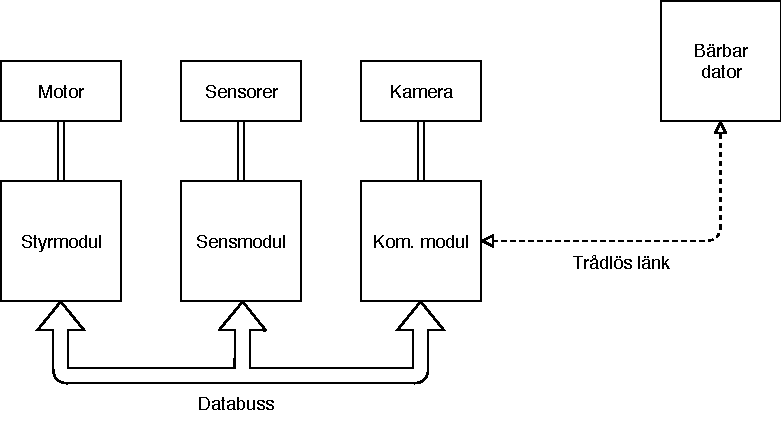
\includegraphics[width=0.4\linewidth]{\figures/blockskiss.pdf}
    \caption{Övergripande bild över systemet och dess moduler. SPI-buss används}
    \label{fig:overview}
\end{figure}

\noindent
Kommunikationsmodulen, vilken består av en Raspberry Pi, fungerar som en
central kommun\-ikations- och beslutsenhet som ansvarar för att ta beslut om
taxins beteende samt hantera kommunikationen mellan modulerna. Styrmodulen,
som består av en motor och en mikrokontroller, står för drift samt reglering
av taxins hastighet och svängradie. Sensormodulen består av en mikrokontroller
samt avståndsmätare och halleffektsensorer monterade på bilens hjul.

\subsection{Sensorer}
Kameran är monterat på ett fäste vid bilens framsida där fästet befinner sig i
en specifik höjd och där man har justerat kamerans lutning utefter behov från
bildbehandlingen. En optiskt avståndsmätare har placerats på bilens framsida
fäst i ett CAD:at fäste. Avståndsmätarenn används till att upptäcka hinder.
Avståndsmätaren skapar avbrott när den har mätt ett distansvärde, detta värde
A/D-omvandlas till ett digitalt 8-bitars värde. Detta värde använder
kommunkationsmodulen för att avgöra när den ska stanna inför hinder. Det finns
även en avståndsmätare placerad vid bilens bakre högersida. Den används till att
avgöra när man har passerat ett hinder vid omkörning. Bilen har 2
halleffektsensorer monterade på chassit där vardera hjul har 10 magneter
monterade. Dessa används till att avgöra antalet rotationer av hjulen och på det
sättet även räkna ut distans körd.

\end{document}
